\section{Sistemas embebidos}
	Los sistemas embebidos son combinaciones de software y hardware con restricciones de recursos que se dedica a una aplicación o parte específica de una aplicación o sistema más grande. Son controlados por una computadora incrustada en ellos, lo que implica que se encuentra dentro del sistema general, oculto a la vista, formando una parte integral de un conjunto mayor. Es probable que dicha computadora sea un microprocesador o microcontrolador.\\
	
	Los sistemas embebidos tienen varias características comunes:
	\begin{itemize}
		\item Un sistema embebido generalmente ejecuta solo un programa, repetidamente.
		\item Su diseño debe ser optimizado para reducir costo y espacio. Contienen sólo los recursos de hardware suficientes para cumplir con  los  requerimientos  de  funcionalidad  de  la  aplicación.
		\item Muchos sistemas embebidos deben reaccionar continuamente a los cambios en el entorno del sistema y deben calcular ciertos resultados sin demora.
	\end{itemize}
	
	
	\subsection{Arquitectura de los sistemas embebidos}
	Un sistema embebido cuenta con varios componentes que permiten que cumpla con las características mencionadas anteriormente. En la figura \ref{fig:MarcoArquiSE} se muestran de forma general la arquitectura de un sistema embebido con todas las partes que lo componen, las cuales se describen a continuación.
	
	\begin{enumerate}
		\item \textbf{Unidad de Procesamiento.} Es el componente encargado de realizar las operaciones de cálculo principales del sistema. Ejecuta código para realizar una determinada tarea y dirige el funcionamiento de los demás elementos que le rodean.
		\item \textbf{Interfaces de entrada.} Establecen la comunicación entre la unidad de procesamiento y el proceso, filtrando, adaptando y codificando de forma comprensible las señales procedentes de los dispositivos de entrada. Algunos de los ejemplos de dispositivos de entrada son: ADC, señales de sensores, módulos de cámara digital, etc. Es importante recalcar que algunos de los dispositivos de entrada se comunican con la unidad de procesamiento haciendo uso de alguna interfaz como SPI, I2C o UART.
		\item \textbf{Interfaces de salida.} Después de que los datos obtenidos mediante los dispositivos conectados a las interfaces de entrada, la unidad de procesamientos decodifica, interpreta, amplifica o procesa los datos obtenidos según sea el caso y los envía mediante las interfaces de salida. En estas interfaces establecen la comunicación entre el sistema embebido y el usuario o dispositivo final. Algunos ejemplos de dispositivos de salida son: módulos WiFi, GSM o Ethernet, los cuales al igual que en las interfaces de entrada, deben ser comunicadas mediante alguna interfaz (SPI, I2C o UART).
		\item \textbf{Memoria.} La memoria esencialmente realiza dos funciones principales dentro de un sistema embebido, una de ellas es proporcionar almacenamiento para el software que se ejecutará, tomando como mínimo la forma de una memoria no volátil que debe conservar su contenido cuando se elimina la alimentación. Otra función principal de la memoria es proporcionar almacenamiento para datos como variables de programa y resultados intermedios, información de estado y cualquier otro dato que pueda crearse durante la operación (memoria volátil).
		\item \textbf{Software.} Los componentes de software dentro de un sistema embebido generalmente abarcan la tecnología que agrega valor al sistema y define qué hace y qué tan bien lo hace. El software puede constar de varios componentes diferentes como: Inicialización y configuración, Sistema operativo o entorno de ejecución, El propio software de aplicaciones, Manejo de errores o Soporte de depuración y mantenimiento.

	\end{enumerate}
	
	\begin{figure}[htbp!]
		\centering
		\fbox{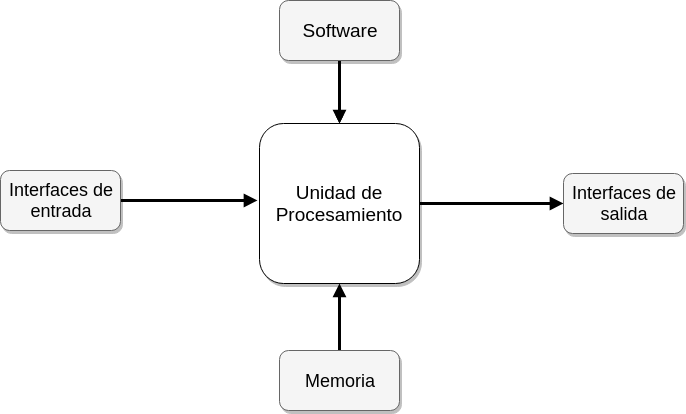
\includegraphics[width=0.8\textwidth]{MarcoTeorico/imagenes/arquitecturaSE.png}}
		\caption{Arquitectura general de un sistema embebido.}
		\label{fig:MarcoArquiSE}
	\end{figure}
%	\TOCHK{Agregar imagen y descripción de su arquitectura}
%	\subsection{Aplicaciones}